\chapter{Latent Semantic Analysis}
\label{sec:lsa}

\begin{summary}
The chapter gives a theoretical overview of \gls{LSA} in the context of its use in this work.
\end{summary}
 
\section{Overview}

\gls{LSA} was first introduced in ~\cite{Dumais88usingLSA} and~\cite{Deerw90_LSA} as a technique for improving information retrieval. Most search engines work by matching words in a user's query with words in documents. Such information retrieval systems that depend on lexical matching have to deal with two problems: synonymy and polysemy. Due to the many meanings which the same word can have, also called polysemy, irrelevant information is retrieved when searching. And as there are different ways to describe the same concept, or synonymy, important information can be missed. \gls{LSA} has been proposed to address these fundamental retrieval problems, having as a key idea dimension reduction technique, which maps documents and terms into a lower dimensional semantic space. \gls{LSA} models the relationships among documents based on their constituent words, and the relationships between words based on their occurrence in documents. By using fewer dimensions that there are unique words, \gls{LSA} induces similarities among words including ones that have never occurred together~\cite{Dumais2006}. There are three basic steps to using \gls{LSA}: parsing text, computing a \gls{SVD}, and mapping queries on the generated semantic space, so that similarities between documents, or queries and documents can be computed.\\
 
\section{Text pre-processing}

Before applying \gls{LSA}, some pre-processing to the texts in the document collection is required. The process of parsing, also called tokenization, is breaking the input text stream into useable tokens. During tokenization, filtering can be applied, i.e. removing HTML tags or other markup, as well as stop words  and punctuation marks. Stop words are such words that don't hold useful information but occur frequently in the texts, and therefore it is sensible to be removed. Examples of stop words are: $ a, an, and, any, some, that, this, to $. \\

An important distinction has to be made between words or terms, and tokens. A term is the class which is used as a unit during parsing, and a token is each occurence of this class. For example, in the sentence: 

\begin{quote}
\textit{CoreMedia CMS is shipped with an installation program for interactive graphical installation and configuration of the software.}
\end{quote}

the term $ installation $ is represented by two tokens. \\

There is no universal way in which to parse a text, and the parsing decisions to address depend on the application in which the text collection will be used. All posterior processing in the following stages of \gls{LSA} will be determined by the parsing. \\

After tokenization, one has to comupute a term - document matrix. Having as rows the terms, and as columns the documents, its elements are number of occurrence of each word in each document. The matrix is sparse, as not all terms occur in all documents.\\

%
% initial sparse matrix A
%
\begin{equation}
A=
\begin{bmatrix}
\label{lsa:sparse_matrix_A}
 a_{11}& a_{12}& \cdots& a_{1n} \\
 \vdots& \vdots& \ddots& \vdots \\ 
 a_{m1}& a_{m2}& \cdots& a_{mn}
\end{bmatrix}\\
\end{equation}\\

The size of the matrix is \text{\bf{m x n}}, where {\bf m} is the number of terms, and {\bf n} is the number of documents in the text collection. Then, the term occurences are transformed into weights using a weight function, such as entropy, term frequency, inverse document frequency. These weights are represented by entries in matrix~\ref{lsa:sparse_matrix_A}, where $ a_{ij} $ gives the weight of term $ i $ in document $ j $. \\

\section{Singular Value Decomposition}

After the initial pre-processing, the generated term-document matrix is decomposed into three matrices by a process called Singular Value Decomposition~(\gls{SVD}). It is a unique decomposition of a matrix into the product of three matrices - $U$ and $V$ are ortonormal matrices, and $S$ is a diagonal matrix with singular values on its diagonal, as in~\ref{lsa:svd}.\\
%
% SVD decomposition in three matrices
%
\begin{equation}\label{lsa:svd}
A=USV^{T}\\
\end{equation}\\

After the initial matrix $A$ is decomposed by \gls{SVD}, all but the highest $k$ valued of $S$ are set to $0$. The resulting reduced matrix is the semantic space of the text collection. A classical example from \cite{Dumais88usingLSA} presenting the truncated \gls{SVD} can be used for displaying dimensionality reduction, and how it affects all three matrices (Figure~\ref{lsa:truncated_svd}).\\

%
% diagram of the truncated SVD
%
\begin{figure}[htbp]
\label{lsa:truncated_svd}
	\centering
	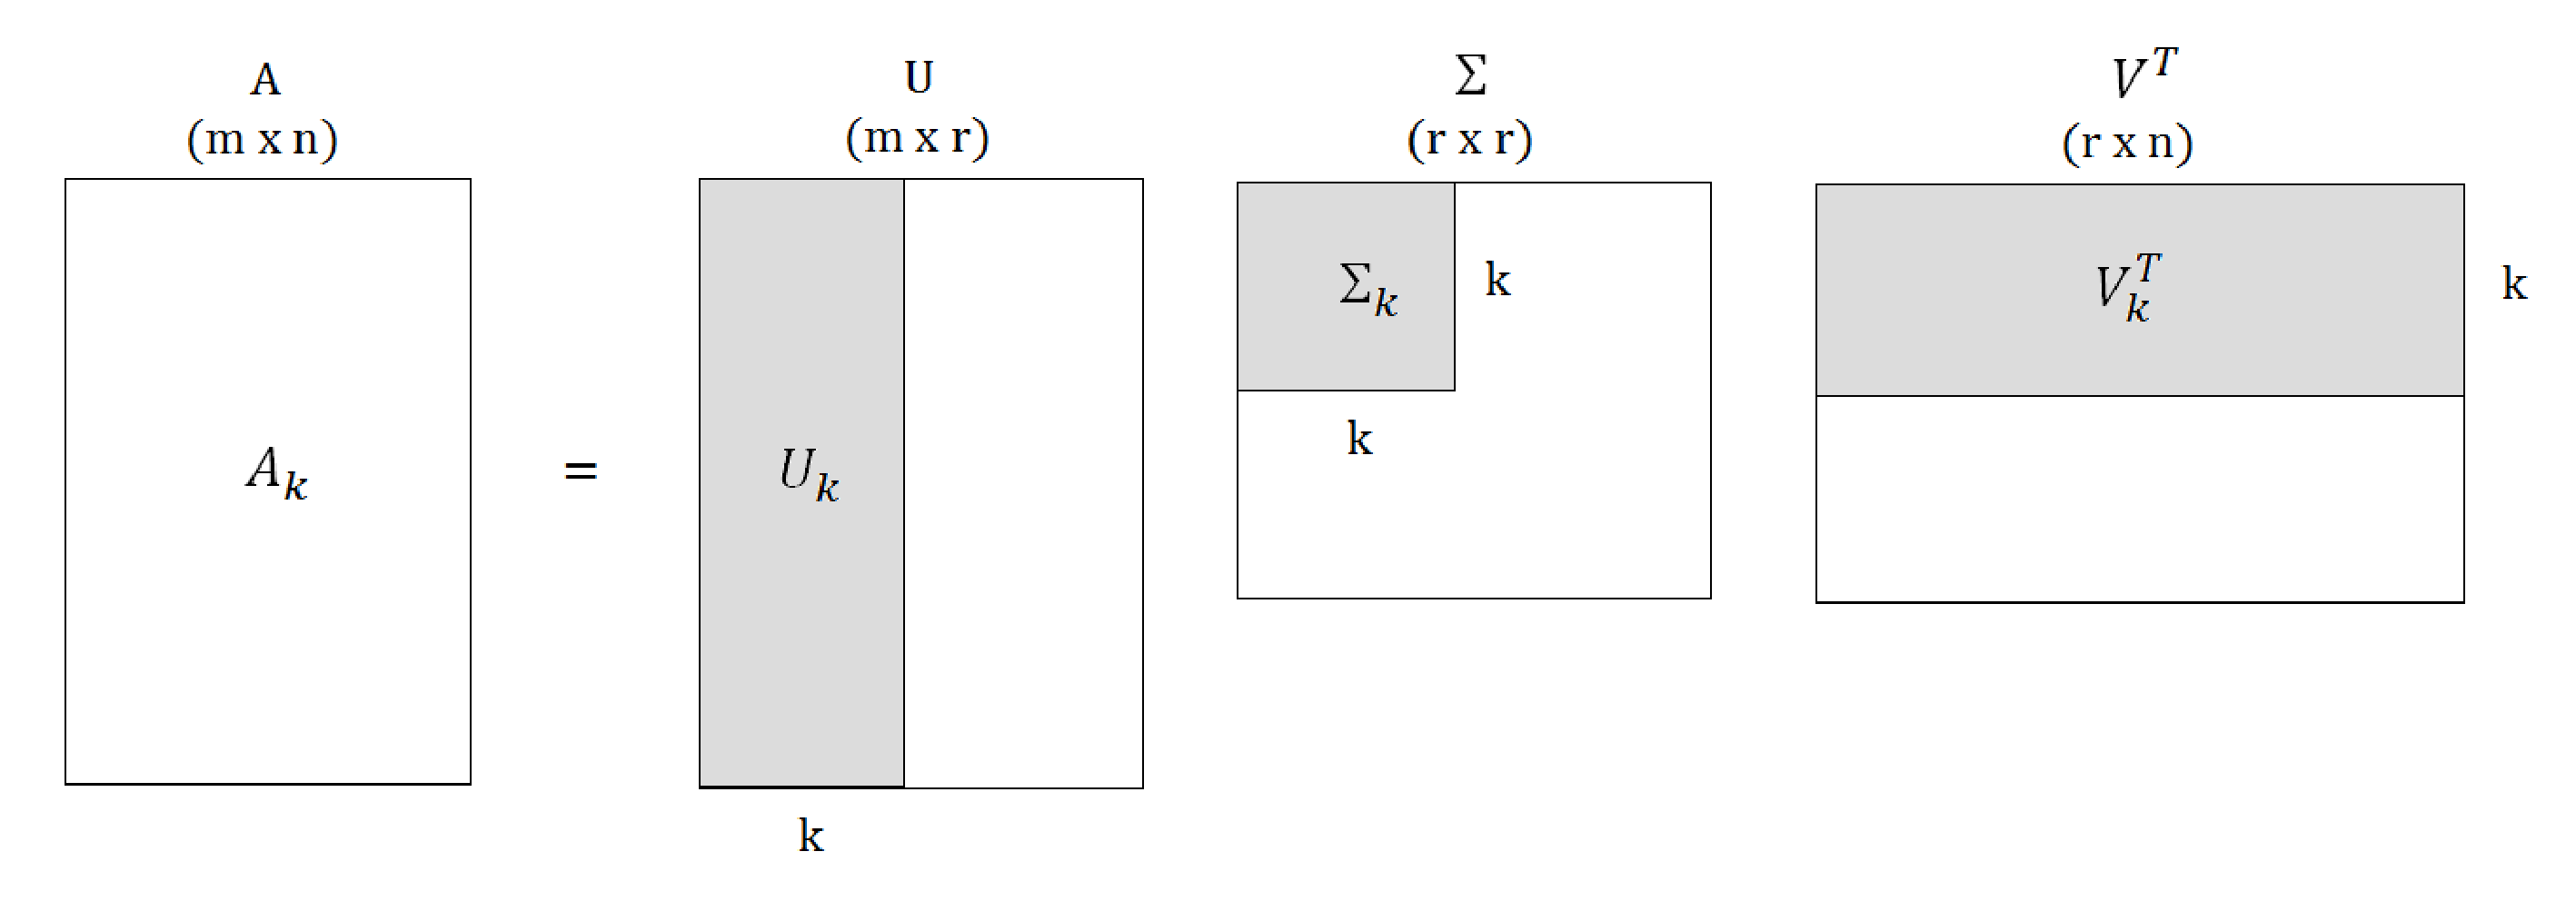
\includegraphics[width=\ScaleIfNeeded]{img/svd} 
 % or [scale=0.5]
	\caption{Diagram of the truncated SVD}
\end{figure}

\gls{LSA} models the relationships between documents based on the words they contain, and the relationships between words based on their occurrence in the documents. By using fewer dimensions that there are unique terms, \gls{LSA} induces similarities among terms including ones that have never occurred together~\cite{Dumais2006}. \gls{SVD} is also a tool for dimensionality reduction, and hence also noise reduction, as it sets to $0$ the lowest term weights. \\

For decomposition of very large matrices, it is important to note that the run time complexity for performing \gls{SVD} is $O(n^2k^3)$, where $n$ is the number of terms, and $k$ is the number of dimensions in semantic space after dimensionality reduction. $k$ is typically a small number between 50 and 350.\\

For more detailed information on \gls{SVD}, please refer to \cite{Berry95usinglinear} and \cite{MatrixCompGolub96}.\\

\section{Query mapping in the semantic space}

The final step of applying \gls{LSA} is to compute similarities between entities in the semantic space. This includes computing similarities between queries and documents in the semantic space. In this case the query $q$ has to be ''translated'' as a document from the semantic space, by using~\ref{lsa:query}.$q^{T}$ is the transposed query vector, $U_{k}$ is the reduced term matrix, and $S_{k}^{-1}$ is the reduced singular values matrix.\\

%
% Query translation for LSA
%
\begin{equation}\label{lsa:query}
q = q^{T}U_{k}S_{k}^{-1}\\
\end{equation}\\

Search in the reduced vector space after \gls{SVD} is done based on a similarity measure and coocurence of the terms within the documents. The decomposition finds the optimal projection into low-dimensional vector space.\\

\section{Factors influencing LSA performance}

Several factors influence the quality of results which LSA delivers. These factors are pre-processing (removal of stop-words, stemming, lemmatization), frequency matrix transformations, choice of dimensionality, choice of similarity measure.\\
A study by Nakov, Popova, Mateev\cite{Nakov_weightfunctions} has summarized the influence of those factors on LSA, and has concluded that...\\

TODO:here give a formula for weighting function, and for similarity measure. Explain citing Nakov's paper why you are using exactly these. \\

There are three main factors that can influence the performance of LSA\cite{Nakov_weightfunctions}\cite{NakovBetterResultsLSI}:\\
\begin{itemize}
\item Frequency matrix transoformations (choice of weighting function)
\item Choice of dimensionality
\item Text preprocessing prior to SVD, choice of similarity measure (???)
\end{itemize}

Further, the choice of dimensionality is dependent upon the matrix transformations performed, as pointed out by Nakov\cite{NakovBetterResultsLSI}.\\

\section{Advantages and drawbacks}

why am i using lsa instead of lda for example?\\

\begin{enumerate}
\item PLSA - characteristics, advantages, disadvantages
\item LDA - characteristics, advantages, disadvantages
\end{enumerate}

\section{Latest development in the field of LSA}
LSAView is a tool for visual exploration of latent semantic modelling, developed at Sandia National Laboratories \cite{CrDuSh09}.\\

at the end- improvements of lsa with the basics explained.\\
